\documentclass[a4paper,12pt]{article}

%Class
	%\documentclass[a4paper,12pt]{article}

%Packages
	\usepackage{amsmath}					% Standard maths
	\usepackage{amssymb}					% Standard maths
	\usepackage{amsthm}						% Standard maths
	\usepackage{thmtools, thm-restate}% Theorem styles
	\usepackage{mathtools}
	\usepackage[newzealand]{babel}% Date/time in British format (yes, I know it says NZ)
	\usepackage{datetime}					% Date/time
	\usepackage{multirow}					% For stacked subscripts
	\usepackage{xcolor}						% For colour!
	\usepackage[normalem]{ulem}		% For strikeout
	\usepackage{isomath}
	\usepackage{fancyhdr}					% For the headers
	\usepackage{mfirstuc}					% For the headers
	\usepackage[hmargin=1in,top=0.8in,bottom=1in]{geometry} % Page margins more reasonable
	\usepackage{graphicx}					% For including graphics
	%\usepackage{float}						% For something
	\usepackage{enumitem}					% For numbering tweaks
	\usepackage{pgfplots}
	\usepackage[margin=15pt,font={footnotesize},labelfont=bf,format=hang]{caption}
\usepackage[margin=15pt,font={footnotesize},labelfont=bf,format=hang]{subcaption}
	\usepackage{url}
	\usepackage[hidelinks]{hyperref}	% For hyperlinks
	\usepackage{breakurl}
	\usepackage{cleveref}
	\usepackage[scaled=.92]{helvet}
	\newbool{show_question}
	\newbool{show_solution}
	\newcommand{\solutioninheading}{\ifbool{show_solution}{: SOLUTIONS}{}}
	\usepackage{pgfplots}
\newcommand{\ep}{\varepsilon}

\makeatletter 
\newcommand\mynobreakpar{\par\nobreak\@afterheading} 
\makeatother

    \newcommand{\question}[3]{
    	\item \textbf{#1} \mynobreakpar \nobreak \medskip % Title
    	%
    	\ifbool{show_question}{\nobreak#2}{} % Question
    	%
    	%
    	\ifbool{show_question}{\ifbool{show_solution}{\par\medskip\textbf{Solution:}}{}}{} % Both
    	\ifbool{show_solution}{#3}{} % Answer
    }			

%MATHEMATICAL SHORTCUTS
%Two and three-part definitions
	\newcommand{\twopartdef}[4]
	{	\left\{
			\begin{array}{ll}
				#1 & \mbox{if } #2 \\
				#3 & \mbox{if } #4
			\end{array}
		\right.}
%	\newcommand{\threepartdef}[6]
%	{	\left\{
%			\begin{array}{ll}
%				#1 & \mbox{if } #2 \\
%				#3 & \mbox{if } #4 \\
%				#5 & \mbox{if } #6
%			\end{array}
%		\right.}
%Blackboard bold	
	\newcommand{\N}{{\mathbb N}} 
	\newcommand{\R}{{\mathbb R}} 
	\newcommand{\C}{{\mathbb C}} 
	%Curly letters
%	\newcommand{\E}{{\mathcal E}}	
%	\newcommand{\F}{{\mathcal F}} 
%	\newcommand{\Null}{{\mathcal N}} 
%	\newcommand{\R}{\mathcal{R}} 
%	\newcommand{\Z}{\mathcal{Z}} 
%Uprights
	\newcommand{\D}{{\mathrm D}}
	\renewcommand{\d}{{\mathrm d}}
%Easy Greeks
%	\def\a{\alpha}
%	\def\g{\gamma}
%	\newcommand{\e}{{\varepsilon}}
%	\newcommand{\la}{{\lambda}}  
%	\newcommand{\om}{{\Omega}}
	\renewcommand{\epsilon}{\varepsilon}
	
%Vector operators
	\def \p {\partial}
	\newcommand{\del}{{\nabla}}
	\newcommand{\grad}{{\nabla}}
    \newcommand{\vdel}{\boldsymbol{\nabla}}
    \newcommand{\vgrad}{\boldsymbol{\nabla}}
    \newcommand{\vnabla}{\boldsymbol{\nabla}}
	\newcommand{\cross}{{\times}}
	\newcommand{\Lap}{{\nabla^2}} 
%Arrows
%	\newcommand{\goesto}[1]{\xrightarrow[#1]{}}
%hats
%	\newcommand{\nhat}{\widehat{\v{n}}}
%	\newcommand{\shat}{\widehat{\v{s}}}
	\renewcommand{\hat}{\widehat}
%Note to self
%	\newcommand{\note}[1]{[\textbf{\textsl{\MakeUppercase{#1}}}]}
	
%Stress tensor
%	\newcommand{\T}{\vg{\sigma}}

% Vectors, quaternions etc.
\renewcommand{\v}[1]{\mathbfit{#1}}      % Generic vector
\newcommand{\vc}[1]{\bm{\mathcal{#1}}}      % vector mathcal
\newcommand{\uv}[1]{\widehat{\mathbfit{#1}}}      % Generic unit vector
\newcommand{\q}[1]{\mathsfbfit{#1}}        % Generic quaternion
\renewcommand{\t}[1]{\mathsfbfit{#1}}	 % Generic tensor
\newcommand{\m}[1]{\mathsfbfit{#1}}	 % Generic matrix
\newcommand{\vu}[1]{\mathbf{#1}}         % Upright vector (for zero vector)
\newcommand{\qu}[1]{\mathbf{#1}}       % Upright quaternion (for zero quaternion)
\newcommand{\tu}[1]{\bm{\mathsf{#1}}}	 % Upright tensor (for zero tensor)

%Real and imaginary
\renewcommand{\Re}{\operatorname{Re}}
\renewcommand{\Im}{\operatorname{Im}}
	
%Non-dim numbers
%	\renewcommand{\Re}{\operatorname{Re}}
%	\newcommand{\Bi}{\operatorname{Bi}}
%	\newcommand{\Fo}{\operatorname{Fo}}
	
%Misc
\DeclareMathSymbol{\Delta}{\mathalpha}{operators}{1} % Keeps Delta upright
\DeclareMathSymbol{\Gamma}{\mathalpha}{operators}{0} % Keeps Gamma upright
	\newcommand{\cosec}{\operatorname{cosec}}
	\newcommand{\cosech}{\operatorname{cosech}}
	\newcommand{\sech}{\operatorname{sech}}
	\newcommand{\tr}{\operatorname{tr}}
	\newcommand{\erf}{\operatorname{erf}}
	\newcommand{\order}{\mathcal{O}}
%	\newcommand{\V}{\mathcal{V}} % 	CurlyV = (Bi V) / (1 + Bi)

% Differentiating 
\newcommand{\fd}[2]{\mathchoice{\frac{\d #1}{\d #2}}{\d #1/\d #2}{\d #1/\d #2}{\d #1/\d #2}}
\newcommand{\fdd}[2]{\mathchoice{\frac{\d^2 #1}{\d #2^2}}{\d^2 #1/\d #2^2}{\d^2 #1/\d #2^2}{\d^2 #1/\d #2^2}}
\newcommand{\fddd}[2]{\mathchoice{\frac{\d^3 #1}{\d #2^3}}{\d^3 #1/\d #2^3}{\d^3 #1/\d #2^3}{\d^3 #1/\d #2^3}}
\newcommand{\fdddd}[2]{\mathchoice{\frac{\d^4 #1}{\d #2^4}}{\d^4 #1/\d #2^4}{\d^4 #1/\d #2^4}{\d^4 #1/\d #2^4}}
\newcommand{\fdn}[3]{\mathchoice{\frac{\d^{#1} #2}{\d #3^{#1}}}{\d^{#1} #2/\d #3^{#1}}{\d^{#1} #2/\d #3^{#1}}{\d^{#1} #2/\d #3^{#1}}}
\newcommand{\pd}[2]{\mathchoice{\frac{\p #1}{\p #2}}{\p #1/\p #2}{\p #1/\p #2}{\p #1/\p #2}}
\newcommand{\pdd}[2]{\mathchoice{\frac{\p^2 #1}{\p #2^2}}{\p^2 #1/\p #2^2}{\p^2 #1/\p #2^2}{\p^2 #1/\p #2^2}}
\newcommand{\pddmixed}[3]{\frac{\p^2 #1}{\p #2 \p #3}}
\newcommand{\pddd}[2]{\frac{\p^3 #1}{\p #2^3}}
\newcommand{\pdn}[3]{\mathchoice{\frac{\p^{#1} #2}{\p #3^{#1}}}{\p^{#1} #2/\p #3^{#1}}{\p^{#1} #2/\p #3^{#1}}{\p^{#1} #2/\p #3^{#1}}}
	
	% Misc
\newcommand{\e}{\mathrm{e}}
\renewcommand{\i}{\mathrm{i}}
\newcommand{\dx}{\,\mathrm{d}x}
\newcommand{\dy}{\,\mathrm{d}y}
\renewcommand{\epsilon}{\varepsilon}
\renewcommand{\Re}{\operatorname{Re}}
\newcommand{\Four}{\mathcal{F}}

\newcommand{\mat}[4]{\begin{pmatrix}#1 & #2 \\ #3 & #4 \end{pmatrix}}

	%Column vectors
	\makeatletter
\newcommand\rcvector[2][\\]{\ensuremath{%
  \global\def\rc@delim{#1}%
    \negthinspace\begin{pmatrix}
      \rc@vector #2,\relax\noexpand\@eolst%
    \end{pmatrix}}}
\def\rc@vector #1,#2\@eolst{%
  \ifx\relax#2\relax
    #1
  \else
    #1\rc@delim
    \rc@vector #2\@eolst%
  \fi}
\makeatother

\newcommand{\colvec}{\rcvector}
\newcommand{\rowvec}{\rcvector}
\renewcommand{\binom}{\rcvector}
	
	%Colours
%	\newcommand{\orange}[1]{{\color{orange} #1 }}
%	\newcommand{\blue}[1]{{\color{blue} #1 }}

%Theorem styles
%	\declaretheoremstyle[headpunct={\:\:\:}, shaded={bgcolor={rgb}{0.9,0.9,0.9}, margin=5pt}]{problem}
%	\declaretheoremstyle[headpunct={\:\:\:}, shaded={rulecolor=black, rulewidth=0.4pt, bgcolor={rgb}{1,1,1}, margin=5pt}]{definition}
%	\declaretheoremstyle[headpunct={\:\:\:}, spaceabove=15pt, notefont=\bf, notebraces={(}{)}]{theorem}
%	\declaretheoremstyle[headpunct={\:\:\:}, numbered=no, spaceabove=15pt, qed={\checkmark}]{solution}
%	
%	\declaretheorem[style=definition,numberwithin=section]{definition}
%	\declaretheorem[numberlike=definition, style=theorem]{theorem}
%	\declaretheorem[numberlike=definition, style=theorem]{lemma}
%	\declaretheorem[numberlike=definition,style=problem]{problem}
%	\declaretheorem[numberlike=definition, style=theorem]{proposition}
%	\declaretheorem[numberlike=definition, style=theorem]{corollary}
%	\declaretheorem[numberlike=definition, style=theorem]{remark}
%	\declaretheorem[numberlike=definition, style=theorem]{example}
%	\declaretheorem[numberlike=definition, style=theorem]{notation}
%	\declaretheorem[style=solution]{solution}

%Depth of display breaks to allow	
	\allowdisplaybreaks[1]

%How deep do we want the Table of Contents to go?	
%	\setcounter{tocdepth}{1}

%Sections
\makeatletter
\renewcommand{\section}{\@startsection
{section}%                   % the name
{1}%                         % the level
{0mm}%                       % the indent
{-\baselineskip}%            % the before skip
{0.5\baselineskip}%          % the after skip
{\normalfont\bfseries}} % the style
\makeatother

% Wavy underline
\makeatletter
\font\sixly=lasyb10 scaled 1200
\def\tinners{\bgroup \markoverwith{\lower8.5\p@\hbox{\sixly \char58}}\ULon}
\makeatother
\newcommand{\answer}[1]{\tinners{\; #1 \;}}

%Setting the footnotes to use *,**,+ etc rather than 1,2,3	
\renewcommand{\thefootnote}{\fnsymbol{footnote}}

%Italic quote environment
%\newenvironment{quoteitalic}{\begin{quote}\itshape}{\end{quote}}

%Heading
\newcommand{\heading}[2]{
\setlength{\parindent}{0pt}
\textbf{MATH3171 (Mathematical Biology III)}

\textbf{YEAR 2025--26, \MakeUppercase{#1} TERM}
\setlength{\parskip}{3ex}

\textbf{\MakeUppercase{#2}}
%
\setlength{\parskip}{2ex}

}

%========================================================================================================================
%DOCUMENT BEGINS HERE!

\setbool{show_question}{true}
\setbool{show_solution}{false}
\begin{document}
%
\heading{Michaelmas}{Problems class 4\solutioninheading}

\ifbool{show_solution}{}{
In this final problems class of term, we will look at two old exam questions which model medical applications. The first considers how quickly wounds heal themselves; and the second looks at vaccine efficacy, marking five years since the announcement of the efficacy of the first Covid vaccines.}

%\ifbool{show_solution}{}{
%  This time in 2020, we had just heard early results showing the efficacy of the Pfizer and Moderna vaccines against the initial Covid strain. Then this time last year, the development of the Omicron variant had us wondering again as to these vaccines' efficacy. In this final problems class of term, we are going to develop our model, first to introduce natural birth and death, and then to introduce a vaccine.
%
%  10 November 2020 in Parliament: (source: \href{https://hansard.parliament.uk/Commons/2020-11-10/debates/FB5296EC-628D-4C17-9C28-4863AC8C07C9/Covid-19Update}{Hansard})
%  \vspace{-0.3cm}
%  \begin{description}
%    \item[Jonathan Ashworth, shadow secretary of state for health and social care:]What is the government’s current working assumption of the proportion of the population that needs to be vaccinated to establish herd immunity and bring $R$ below 1?
%    \item[Matt Hancock, secretary of state for health and social care:][Pre-jungle stardom] The honest truth to that question is that we do not know what proportion of the population the vaccination needs to reach in order for it to stop the epidemic.
%  \end{description}
%  \vspace{-0.3cm}
%  We will try to answer this question for the model we develop.
%}

\begin{enumerate}[label={\bf \arabic{*}.\;}, ref={\arabic{*}},itemsep=3ex, left=0ex]

\question{Travelling waves in skin repair (Exam 2022, section B)}
{ % Question
    A model of wound healing in one spatial dimension is given by
    \begin{equation}
        \pd{u}{t}=\pdd{u}{x}-u\log\left(\frac{u+a}{K}\right),
        \label{wound-healing}
    \end{equation}
    where $u(x,t)$ is the density of healthy tissue at position $x$ and time $t$; and where $a$ and $K$ are positive constants, with $0<a<K$.
    \begin{enumerate}
    \item Consider first the homogeneous form of (\ref{wound-healing}). Find the equilibria and determine their stability in this case.
    \item Describe qualitatively the full model, (\ref{wound-healing}). In what way is it different to that described by the Fisher--Kolmogorov equation?    
    \item We are going to look for travelling wave solutions, i.e.\ solutions of the form $u(z)$, where $z=x-ct$ and $c>0$. Given the stability of the equilibria in the homogeneous system, suggest suitable boundary conditions for $u(z)$ at $z=\pm \infty$, explaining your choice.
    \item Now write (\ref{wound-healing}) for $u(z)$, and by performing a linear stability analysis, determine the stability of the homogeneous equilibria. Given that waves travel at their lowest possible speed, determine the wavespeed, $c$.
    \item Consider now a wound which is initially of length $L$, i.e.\ as in the diagram below, where $u^*$ is the value of the nonzero homogeneous equilibrium of (\ref{wound-healing}):
    
    \begin{center}
        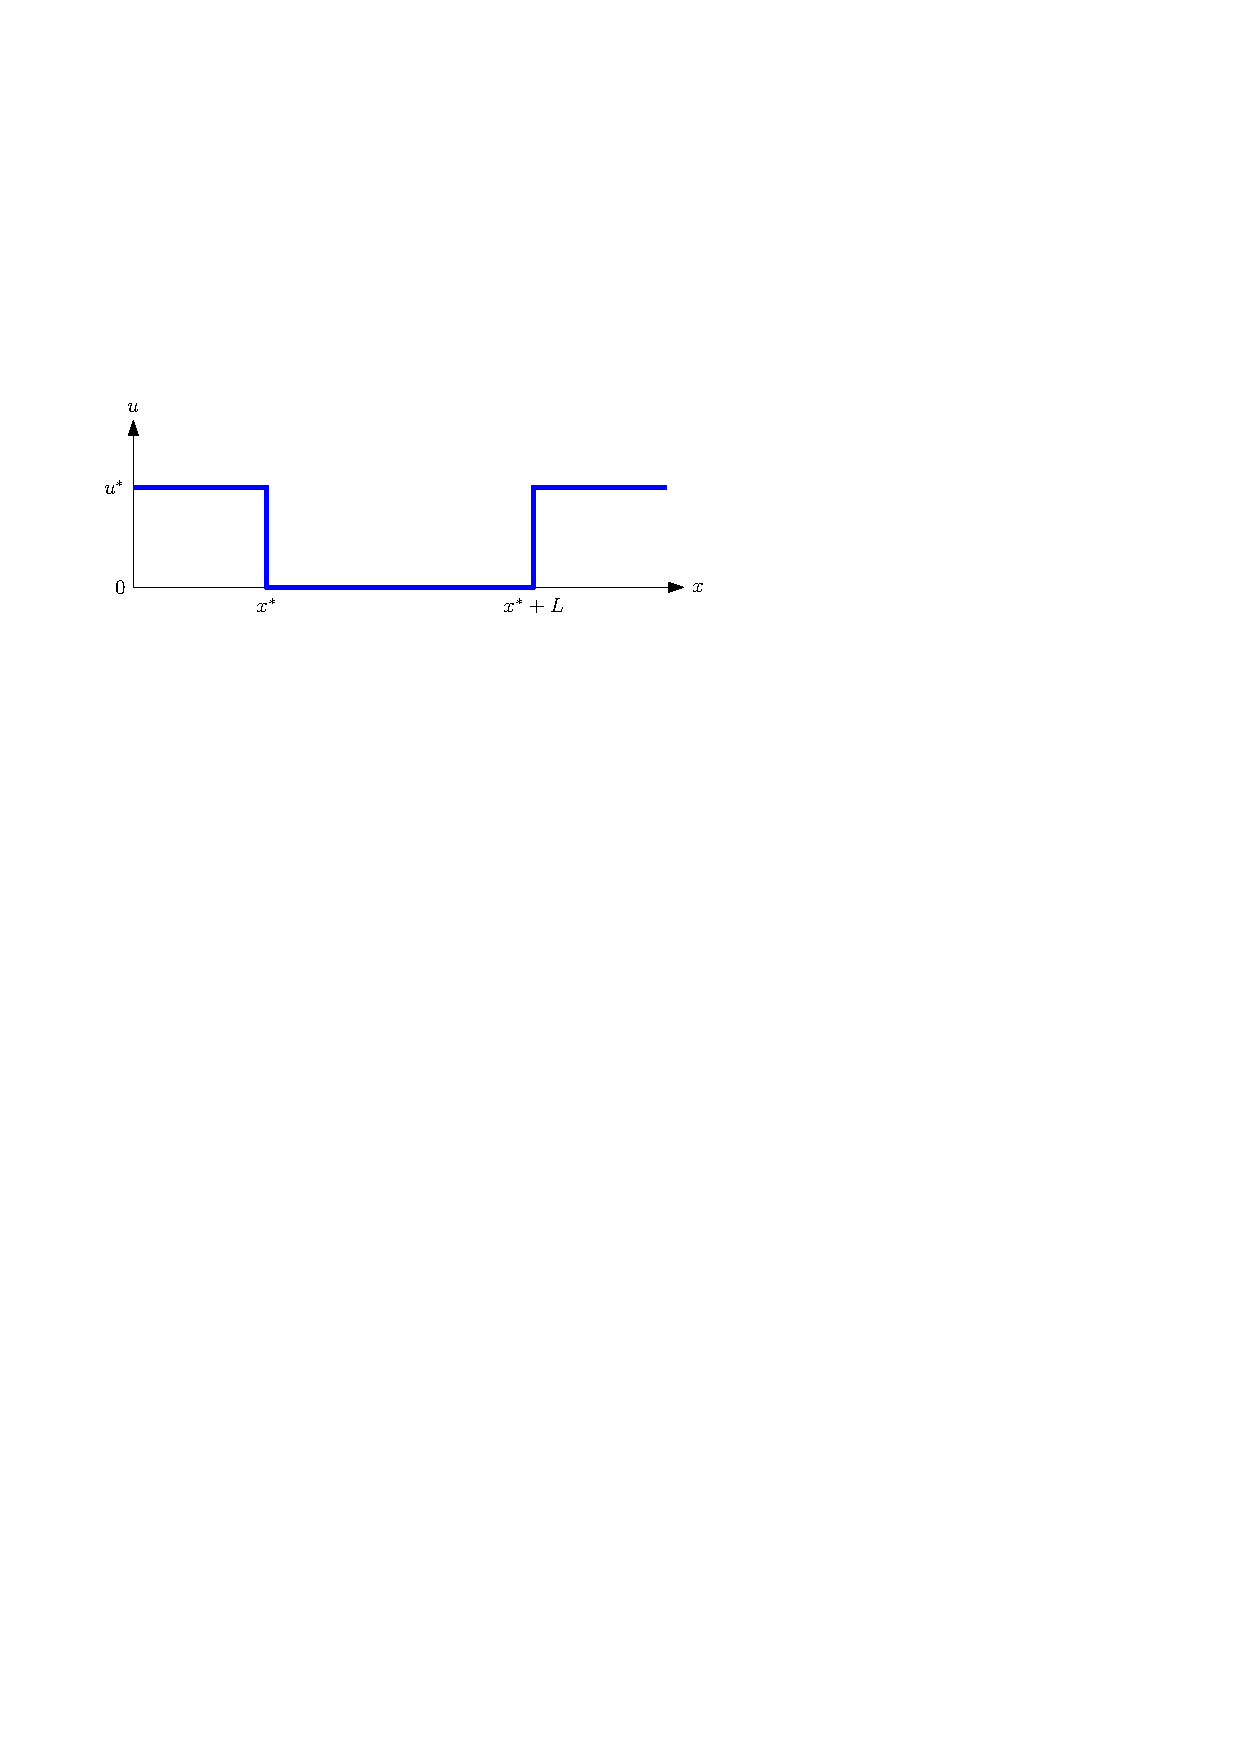
\includegraphics[scale=1.2]{wound2}
    \end{center}
    
    Illustrating your answer with sketches of $u(x,t)$ for increasing $t$, explain what you expect to happen for subsequent times and determine approximately how long it will take for the wound to heal.
    \end{enumerate}
}{ % Solution
\begin{enumerate}
    \item %Q7.1
    The homogeneous equation is
    \begin{equation*}
        \fd{u}{t} = -u\log\left(\frac{u+a}{K}\right).
    \end{equation*}
    The equilibria are at $u=0$ and $u=K-a$.
    
    Their stability can be determined graphically:
    \begin{center}
        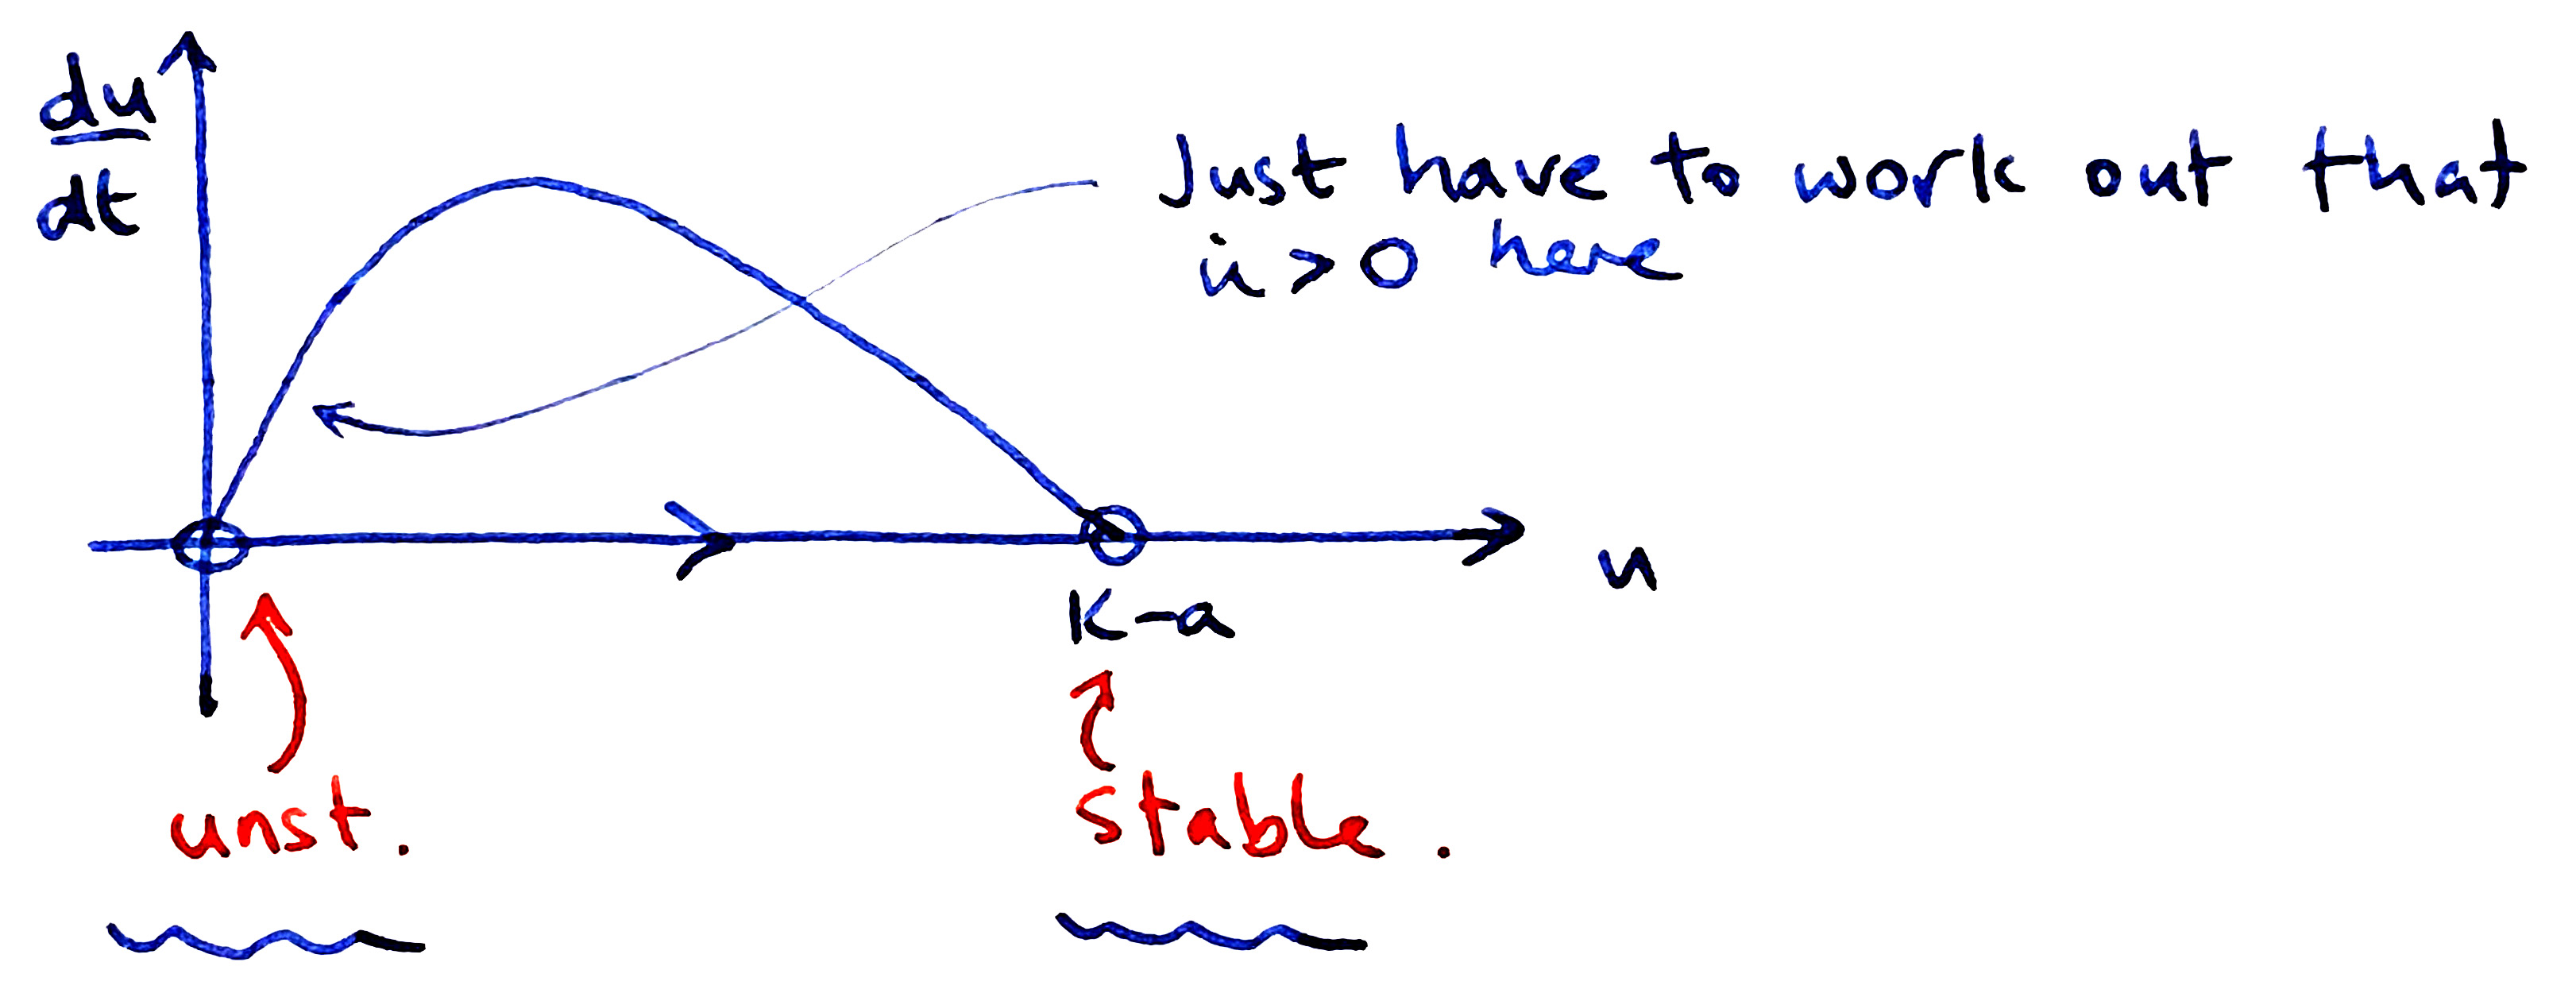
\includegraphics[width=14cm]{wave-stability.jpg}
    \end{center}
    or spotting that for $0<u\ll1$, $\fd{u}{t}>0$ because $\log(a/K)<0$ since $a<K$. So $u=0$ is unstable and since the stability of 1D systems alternates, $u=K-a$ must be stable.
    %
    \item %Q7.2
    Description of the model:
    \begin{itemize}
        \item diffusion with a growth term, which has a carrying capacity $u=K-a$,
        \item similar to FK (see graph above) in shape and having a carrying capacity, but FK is logistic, `$+u(1-u)$'.
    \end{itemize}
    %
    \item %Q7.3
    Argument of the form:
    \begin{itemize}
        \item Expect the stable equilibrium, $u=K-a$, to expand, so the wave will travel away from this.
        \item A wave of the form $z=x-ct$ moves to the \emph{right}.
        \item Therefore pick
        \begin{equation*}
            u(-\infty) = K-a, \quad u(\infty)=0.
        \end{equation*}
    \end{itemize}
    %
    \item 
    Substituting in $z=x-ct$, we have
    \begin{equation*}
        \pd{u}{t} = -c\fd{u}{z} \quad \text{and} \quad \pdd{u}{x} = \fdd{u}{z},
    \end{equation*}
    so
    \begin{equation*}
        -c \fd{u}{z} = \fdd{u}{z} - u\log\left(\frac{u+a}{K}\right).
    \end{equation*}
    To perform the linear stability analysis, let $v = \fd{u}{z}$ then
    \begin{align*}
        \fd{u}{z} &= v,\\
        \fd{v}{z} &= -cv+u\log\left(\frac{u+a}{K}\right).
    \end{align*}
    The Jacobian is
    \begin{equation*}
        \m{J} = \begin{pmatrix}
            0 & 1 \\ \log \left(\frac{u+a}{K}\right) + \frac{u}{u+a} & -c
        \end{pmatrix},
    \end{equation*}
    where the bottom-left entry is worked out as
    \begin{align*}
        \fd{}{u}\left[u\log\left(\frac{u+a}{K}\right)\right] &= \log \left(\frac{u+a}{K}\right)+u\frac{K}{u+a}\frac{1}{K} \\
        &= \log \left(\frac{u+a}{K}\right)+\frac{u}{u+a}.
    \end{align*}
    Evaluated at $(0,0)$, the Jacobian is
    \begin{equation*}
        \m{J} = \begin{pmatrix}
            0 & 1 \\ \log\frac{a}{K} & -c
        \end{pmatrix}.
    \end{equation*}
    The eigenvalue equation is therefore
    \begin{align*}
        -\lambda(-\lambda-c)-\log\frac{a}{K} &= 0 \\
        \implies \lambda^2 + c\lambda - \log\frac{a}{K} &= 0,
    \end{align*}
    and hence
    \begin{equation*}
        \implies \lambda = \frac{1}{2}\left( -c \pm \sqrt{\vphantom{\frac{a}{K}}\smash[b]{c^2 + 4\underbrace{\log\frac{a}{K}}_{<0}}} \right).\vspace{0.4cm}
    \end{equation*}
    This is therefore a stable node (two negative, real eigenvalues) if
    \begin{equation}
        c^2 > -4\log\frac{a}{K},\label{wave-speed}
    \end{equation}
    else it is a spiral (complex eigenvalues).
    
    The Jacobian, evaluated at $(K-a,0)$, is
    \begin{equation*}
        \m{J} = \begin{pmatrix}
            0 & 1 \\ \frac{K-a}{K} & -c 
        \end{pmatrix},
    \end{equation*}
    and hence
    \begin{equation*}
        \implies \lambda = \frac{1}{2}\left( -c \pm \sqrt{\vphantom{\frac{K-a}{K}}\smash[b]{c^2 + 4\underbrace{\frac{K-a}{K}}_{>0}}} \right).\vspace{0.4cm}
    \end{equation*}
    The eigenvalues are real, with different sign. This is therefore a saddle point.
    
    A spiral is not possible, as that would mean negative $u$, which is unphysical. We therefore conclude \cref{wave-speed} is true, and, further, since waves travel at their lowest possible speed, 
    \begin{equation*}
        c = 2\sqrt{\log\frac{K}{a}}.
    \end{equation*}
    %
    \item %Q7.5
    Expect $u(x,t)$ to develop like:
    
    \begin{center}
        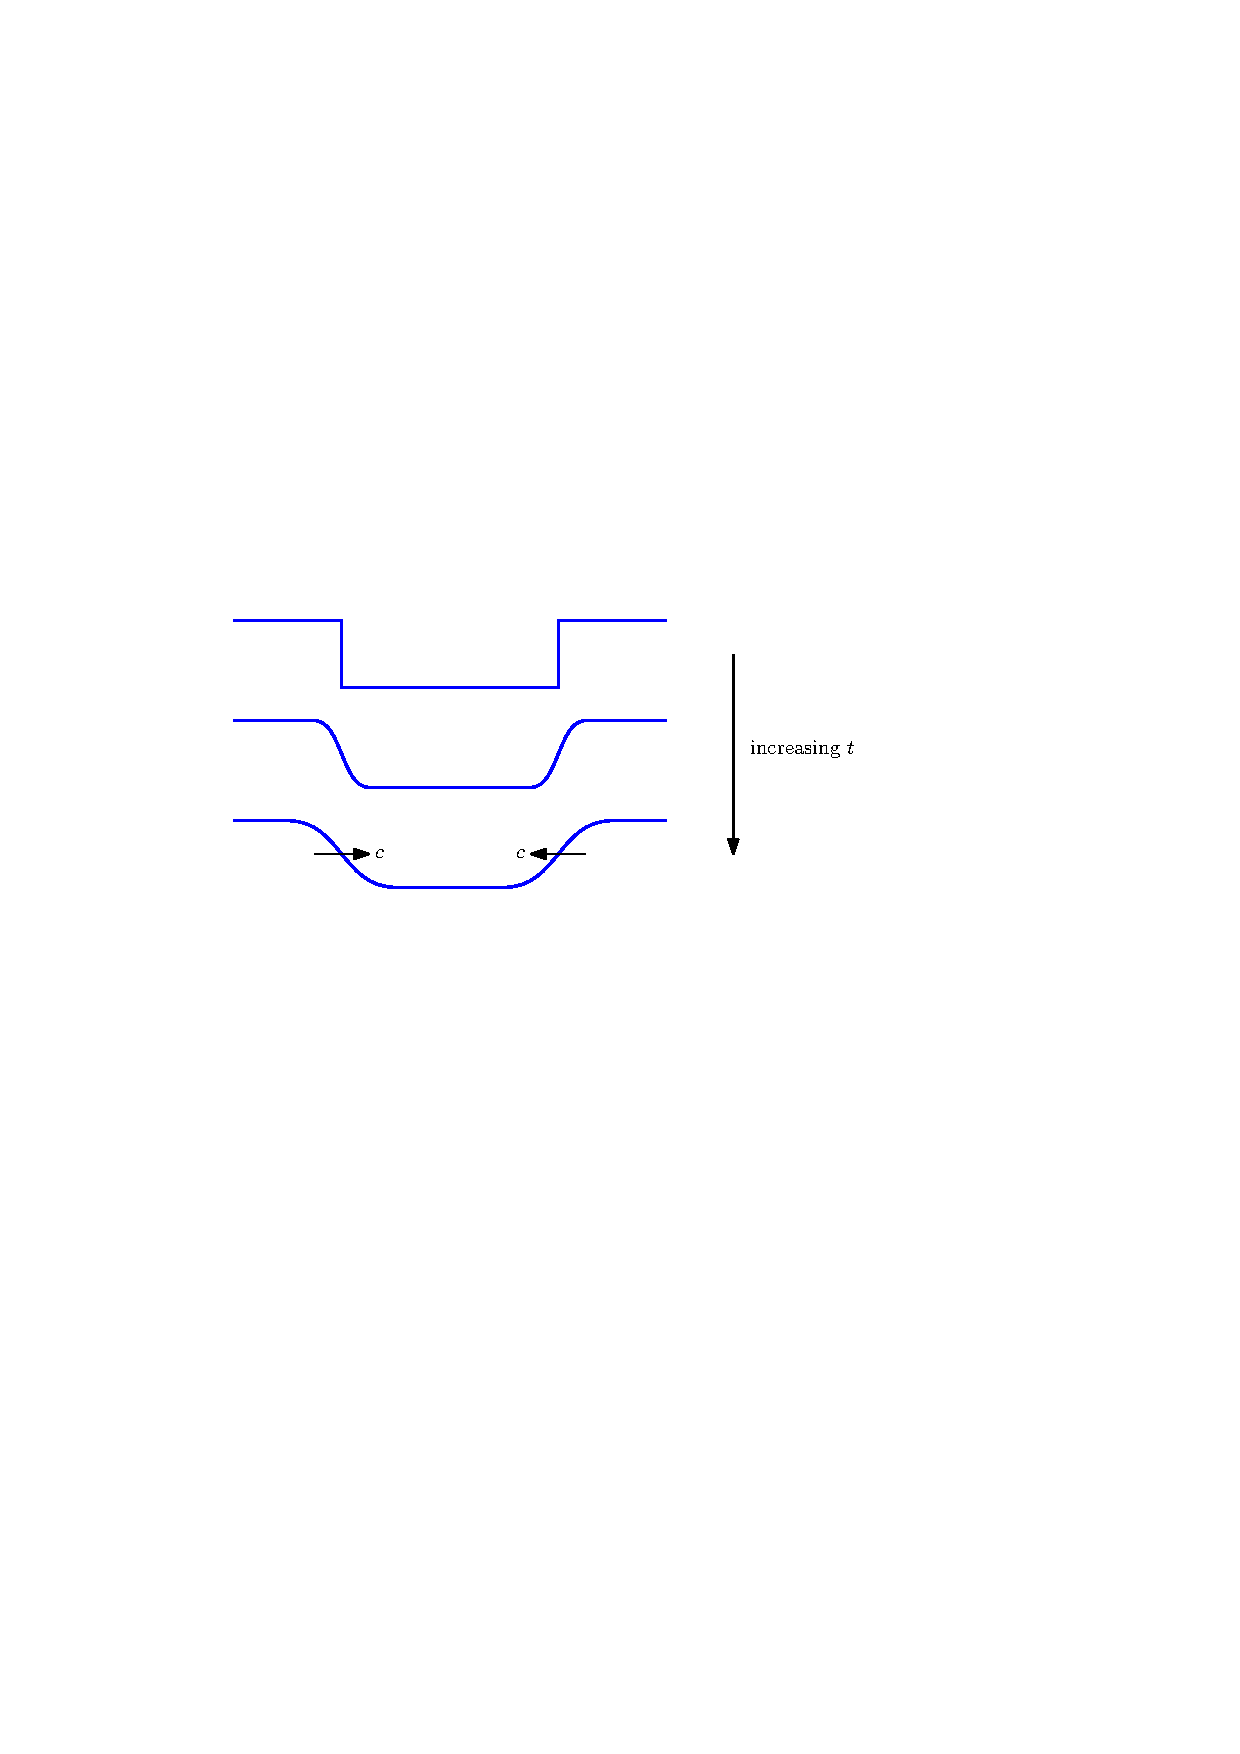
\includegraphics[scale=1.2]{wound.pdf}
    \end{center}
    
    with a closure time of approximately
    \begin{equation*}
        \frac{L/2}{c} = \frac{L}{4\sqrt{\log(K/a)}}.
    \end{equation*}
    
\end{enumerate}

}
\newpage
\question{Disease modelling with vaccination (Exam 2022, section B)}
{
\begin{quote}
  \textbf{Parliament, 10 November 2020} (\href{https://hansard.parliament.uk/Commons/2020-11-10/debates/FB5296EC-628D-4C17-9C28-4863AC8C07C9/Covid-19Update}{Hansard}):
  \vspace{-0.1cm}
  \begin{description}
    \item[\rm\itshape Jonathan Ashworth, shadow secretary of state for health and social care:]What is the government’s current working assumption of the proportion of the population that needs to be vaccinated to establish herd immunity and bring $R$ below 1?
    \item[\rm\itshape Matt Hancock, secretary of state for health and social care:] The honest truth to that question is that we do not know what proportion of the population the vaccination needs to reach in order for it to stop the epidemic.
  \end{description}
\end{quote}
Consider the following extension of the SIR model for an infectious disease, where susceptible individuals are vaccinated at a rate $\nu$,
\begin{align}
\fd{S}{t} &=\alpha R - \beta I S - \nu S, \label{s-eq}\\
\fd{I}{t} &= \beta I S - \gamma I, \label{i-eq}\\
\fd{R}{t} &= \gamma I - \alpha R + \nu S,\nonumber
\end{align}
where $\alpha,\beta,\gamma,\nu$ are all positive constants, and $S(t),I(t),R(t)\geq 0$ to be permissible.
\begin{enumerate}
	\item Show that $N=S+I+R$ is constant and use this to eliminate $R$ from (\ref{s-eq}). Explain why, from now on, we only need to consider the subsystem formed of equations (\ref{s-eq}) and (\ref{i-eq}).
	\item Give an interpretation of the constants $\alpha,\beta,\gamma,N$. What would be suitable units for these constants?	
	\item It is proposed that this could be an appropriate model for the spread of Covid-19. Is this a suitable model for this problem? Give three clear arguments, which can be in favour of this as a suitable model, or against its suitability. Your three arguments do not have to argue the same way. %No way for people to die!! 
	\item 
	\begin{enumerate}[label=(\roman*)]
		\item Find the values of $S$ and $I$ at the two equilibria of the system.
		\item The disease is eradicated if the disease-free equilibrium is the only possible stable equilibrium and the endemic equilibrium does not exist. Perform a linear stability analysis on both equilibria of the system and show that the disease is eradicated if $R^*<1$, where you should define the constant $R^*$.
		\item Define $R_0$ as the value of $R^*$ in the absence of vaccination (i.e.\ when $\nu=0$): in this way, $R_0$ can be seen as an inherent property of the disease. Rearrange the statement $R^*<1$ to find the condition on the vaccination rate, $\nu$, for the disease to be eradicated in terms of $R_0$.
	\end{enumerate}
	\item You are now asked to present the same argument graphically. Draw a phase portrait of $I$ against $S$ and, by moving the nullclines on your portrait, show how the existence of the endemic equilibrium depends on the vaccination rate, $\nu$, and the value of $R_0$. You do not need to explicitly draw trajectories to make this argument.
\end{enumerate}
}
{
\begin{enumerate}
    \item %Q8.1
    We have that
    \begin{align*}
        \fd{N}{t} &= \fd{S}{t} + \fd{I}{t} + \fd{R}{t}\\
        &= (\alpha R - \beta I S-\nu S) + (\beta I S - \gamma I) + (\gamma I - \alpha R + \nu S) \\
        &= 0.
    \end{align*}
    Eliminating $R$, our system becomes
    \begin{align*}
        \fd{S}{t} &= \alpha(N-S-I)-\beta IS-\nu S,\\
        \fd{I}{t} &= \beta IS - \gamma I.
    \end{align*}
    We can lose the equation for $\fd{R}{t}$ since $\fd{S}{t}$ and $\fd{I}{t}$ are independent of $R$, and because 
    \begin{equation*}
        \fd{R}{t} = -\fd{S}{t} - \fd{I}{t}
    \end{equation*}
    anyway.
    %
    \item %Q8.2
    Interpretation:
    \begin{itemize}
        \item $\alpha$: rate at which immunity wears off; any unit that fits the dimension of $\text{time}^{-1}$,
        \item $\beta$: infection rate; $\text{people}^{-1}\text{time}^{-1}$, 
        \item $\gamma$: recovery rate (possibly death rate, but dubious since it is possible to leave the group $R$); $\text{time}^{-1}$.
    \end{itemize}
    %
    \item %Q8.3
    Example arguments [students should provide three]:
    \begin{itemize}
        \item no because there is no incubation period (as in an SEIR model),
        \item no because dead people cannot be reinfected
        \item no because vaccination doesn't necessarily stop infection, it may just reduce the rate of infection
        \item no because no spatial dependence
        \item yes because it captures the general shape of epidemic `waves'
    \end{itemize}
    %
    \item %Q8.4
    \begin{enumerate}[label=(\roman*)]
        \item %Q8.4(i)
        Equilibria are where
        \begin{align}
            0 &= \alpha(N-S-I)-\beta IS - \nu S, \label{s-null} \\
            0 &= \beta IS - \gamma I. \label{i-null}
        \end{align}
        \Cref{i-null} gives us
        \begin{equation*}
            I = 0 \quad \text{or} \quad S = \frac\gamma\beta.
        \end{equation*}
        If $I=0$ then \cref{s-null} gives us
        \begin{align*}
            0 &= \alpha(N-S)-\nu S \\
            \implies \alpha N &= (\alpha+\nu)S \\
            \implies S &= \frac{\alpha}{\alpha+\nu}N.
        \end{align*}
        And if $S = \gamma/\beta$ then
        \begin{align*}
            0 &= \alpha\left( N - \frac\gamma\beta - I \right) - I \gamma - \frac{\nu \gamma}{\beta} \\
            \implies \alpha N - \frac{\alpha \gamma}{\beta} - \frac{\gamma\nu}{\beta} &= I(\alpha + \gamma)\\
            \implies \alpha N - (\alpha + \nu)\frac\gamma\beta &= I(\alpha + \gamma)\\
            \implies I &= \frac{\alpha \beta N-(\alpha+\nu)\gamma}{\beta(\alpha+\gamma)}.
        \end{align*}
        The two equilibria are therefore
        \begin{equation*}
            \left(\frac{\alpha N}{\alpha + \nu}, 0\right) \quad \text{and} \quad \left(\frac{\gamma}{\beta}, \frac{\alpha \beta N - (\alpha+\nu)\gamma}{\beta(\alpha+\gamma)} \right) \eqqcolon (S^*,I^*).
        \end{equation*}
        %
        \item %Q8.4(ii)
        The Jacobian is
        \begin{equation*}
            \m{J} = \begin{pmatrix}
                -\alpha-\beta I - \nu & - \alpha - \beta S \\
                \beta I & \beta S - \gamma
            \end{pmatrix}.
        \end{equation*}
        Evaluated at $\displaystyle\left(\frac{\alpha N}{\alpha + \nu},0\right)$, it is
        \begin{equation*}
            \begin{pmatrix}
                - \alpha - \nu & - \alpha - \frac{\beta \alpha N}{\alpha + \nu} \\
                0 & \frac{\beta \alpha N}{\alpha + \nu} - \gamma
            \end{pmatrix}.
        \end{equation*}
        The eigenvalues are
        \begin{equation*}
            -\alpha-\nu < 0 \quad \text{and} \quad \frac{\beta\alpha N}{\alpha+\nu} - \gamma.
        \end{equation*}
        So we can say the eigenvalue at $\displaystyle\left(\frac{\alpha N}{\alpha + \nu},0\right)$ is unstable if $\displaystyle\frac{\beta\alpha N}{\alpha+\nu} > \gamma$.
        
        For the endemic equilibrium, $(S^*,I^*)$, use the trace and determinant method.
        \begin{align*}
            \tr\m{J} &= \alpha - \beta I^* - \nu + \beta S^* - \gamma \\
            &= - \alpha - \beta I^* - \nu < 0.
        \end{align*}
        And the determinant, noting that the bottom-right entry of the Jacobian is 0, is
        \begin{align}
            \det\m{J} &= 0 - (-\alpha-\gamma)(I^*\beta) \\
            &= (\alpha+\gamma)I^*\beta > 0.
        \end{align}
        Since $\tr\m{J} < 0$ and $\det\m{J} > 0$, we conclude that $(S^*,I^*)$ is always stable if it exists.
        
        Further, $(S^*,I^*)$ exists if 
        \begin{align*}
            \alpha \beta N - (\alpha + \nu)\gamma &> 0 \\
            \implies \left(\frac{\alpha}{\alpha+\nu}\right)\beta N &> \gamma,
        \end{align*}
        which is the same condition.
        
        The disease is therefore eradicated if
        \begin{equation}
            R^* \coloneqq \frac{\alpha}{\alpha+\nu} \frac{\beta N}{\gamma} < 1. \label{r-star}
        \end{equation}
        %
        %
        \item %Q8.4(iii)
        From \cref{r-star}, we define
        \begin{equation*}
            R_0 = \frac{\beta N}{\gamma}, 
        \end{equation*} and therefore have
        \begin{align*}
            \frac{\alpha}{\alpha+\nu}R_0 < 1 & \implies \alpha R_0 < \alpha + \nu \\
            &\implies \alpha(R_0 - 1) < \nu.
        \end{align*}
    \end{enumerate}
    %
    % Q8.5
    \item
    Phase portrait:
    \begin{center}
        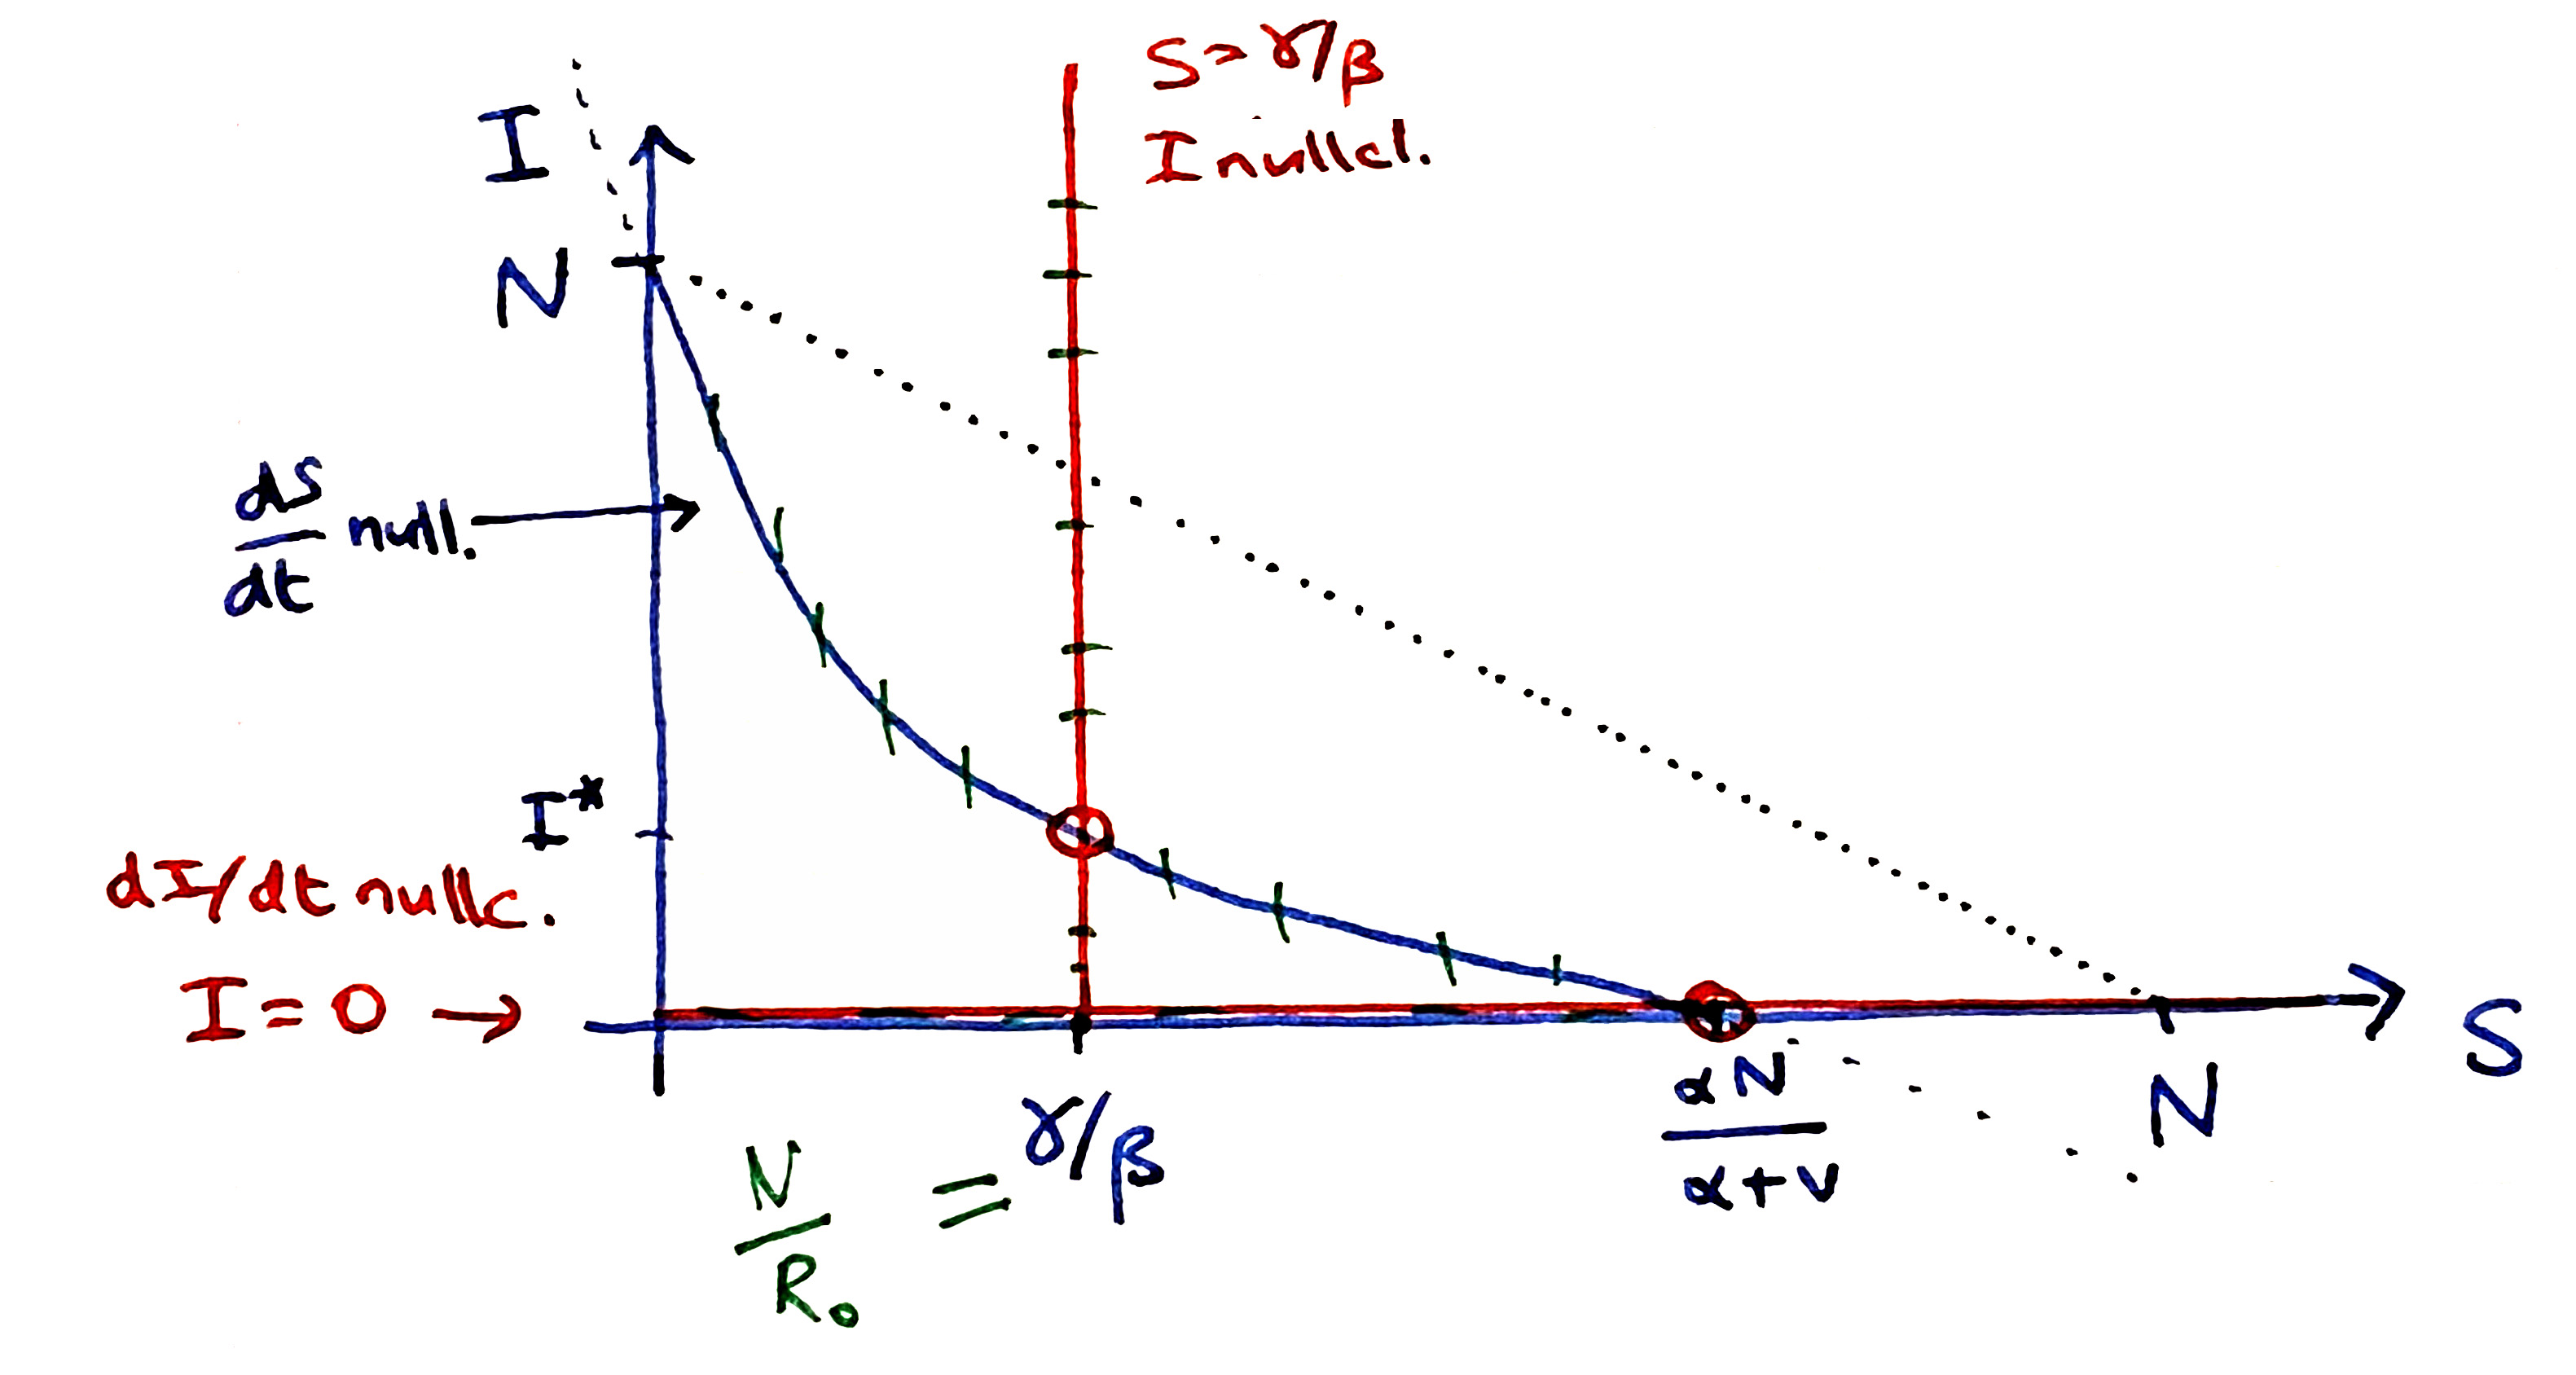
\includegraphics[width=13cm]{sir-graph.jpg}
    \end{center}
    
    The $I$ nullclines are $I=0$ and $S=\gamma/\beta$.
    
    The $S$ nullcline is where
    \begin{align*}
        0 &= \alpha N - \alpha S - \alpha I - \beta I S - \nu S \\
        \implies I(\alpha + \beta S) &= \alpha(N-S)-\nu S \\
        \implies I &= \frac{\alpha N-(\alpha+\nu)S}{\alpha + \beta S}.
    \end{align*}
    This is awkward to plot but notice that
    \begin{equation*}
        I(0) = N \quad \text{and} \quad I\left(\frac{\alpha N}{\alpha + \nu}\right) = 0.
    \end{equation*}
    You can also notice
    \begin{itemize}
        \item for small $S$, $I$ looks linear,
        \item for large $S$, $I$ looks constant,
    \end{itemize}
    which implies the shape in the picture.
    
    As for how the existence of the endemic equilibrium depends on $\nu$ and $R_0$:
    \begin{itemize}
        \item the equilibrium exists where the $S$ and $I$ nullclines cross,
        \item the $I$ nullcline is at $\gamma/\beta = N/R_0$,
        \item changing $R_0$ shifts the $I$ nullcline left and right,
        \item changing $\nu$ squeezes the $S$ nullcline horizontally,
        \item it is possible to eradicate the disease by increasing $\nu$ or decreasing $R_0$.
    \end{itemize}
    
\end{enumerate}
}

%    % Q1
%    \question{SIR with natural birth and death}
%    { % Question
%      In the first two problems classes, we have been working on the popular SIR disease model:
%      \begin{align}
%        \fd{S}{t} &= - \beta I S, \\
%        \fd{I}{t} &= \beta I S - \gamma I, \\
%        \fd{R}{t} &= \gamma I, \\
%        N &= S + I + R.
%      \end{align}
%      We now add in natural birth and death. We haven't added this in so far: under what circumstances might that be OK? Let's assume that everyone can reproduce and that the new offspring enter the model as susceptible. Let's also assume that natural death (i.e.\ death unrelated to this disease) affects everybody equally.
%      \begin{enumerate}[label=(\alph*)]
%        \item Add new terms to the original SIR system to model this new situation.
%        \item In order to have a constant population ($\fd{N}{t} = 0$), what must we assume about the birth and death rates?
%        \item Find the equilibria of this new model.
%        \item By considering the sub-system consisting of the equations for $\fd{S}{t}$ and $\fd{I}{t}$, write down the Jacobian and perform a linear stability analysis on these equilibria. Show that $R_0$ in this new model is
%          \begin{equation}
%            R_0 = \frac{N\beta}{\gamma + \mu},
%          \end{equation}
%          where $\mu$ is the rate of birth and death.
%      \end{enumerate}
%    }
%    { % Solution
%      \begin{enumerate}[label=(\alph*)]
%        \item Our new system is
%          \begin{align}
%            \fd{S}{t} &= \nu N - \beta I S - \mu S, \label{S1}\\
%            \fd{I}{t} &= \beta I S - \gamma I - \mu I, \label{I1}\\
%            \fd{R}{t} &= \gamma I - \mu R, \\
%            N &= S + I + R.
%          \end{align}
%        \item We have to assume they are equal, i.e.\ $\mu=\nu$.
%        \item The two equilibria, from manipulating \cref{S1,I1} when $\fd{S}{t}=\fd{I}{t} = 0$, are
%          \begin{equation}
%            (S_0,I_0) = (N,0) \quad \text{and} \quad (S_0,I_0) = \left( \frac{\mu+\gamma}{\beta}, \frac{\mu}{\beta}\left[ \frac{N\beta}{\mu+\gamma} - 1 \right] \right).
%          \end{equation}
%          The first equilibrium is the disease-free equilibrium; the second the endemic equilibrium.
%        \item The Jacobian is
%          \begin{equation}
%            \m{J} =
%            \begin{pmatrix}
%              -(\beta I + \mu) & -\beta S \\
%              \beta I & \beta S - \gamma - \mu
%            \end{pmatrix}.
%          \end{equation}
%          At the disease-free equilibrium, $(S_0,I_0) = (N,0)$, we have
%          \begin{equation}
%            \m{J} =
%            \begin{pmatrix}
%              -\mu & -\beta N \\
%              0 & \beta N - \gamma - \mu
%            \end{pmatrix}.
%          \end{equation}
%          This gives eigenvalues
%          \begin{equation}
%            \lambda_1 = -\mu < 0, \quad \lambda_2 = \beta N - \gamma - \mu.
%          \end{equation}
%          The second eigenvalue is negative, and therefore this equilibrium is stable, if $\gamma+\mu > \beta N$, i.e.\
%          \begin{equation}
%            \frac{N \beta}{\mu + \gamma} < 1.
%          \end{equation}
%          This gives us our definition for $R_0$:
%          \begin{equation}
%            R_0 = \frac{N \beta}{\mu + \gamma}.
%          \end{equation}
%          Meanwhile, at the endemic equilibrium,
%          \begin{equation}
%            (S_0,I_0) = \left( \frac{\mu+\gamma}{\beta}, \frac{\mu}{\beta}\left[ \frac{N\beta}{\mu+\gamma} - 1 \right] \right),
%          \end{equation}
%          we have
%          \begin{align}
%            \tr\m{J} &= -(\beta I + \mu) + \beta S - \gamma - \mu \\
%            &= -[\mu(R_0 - 1) + \mu] + (\mu + \gamma) - \gamma - \mu \\
%            &= -\mu R_0 < 0,
%          \end{align}
%          and
%          \begin{align}
%            \det\m{J} &= -(\beta I + \mu)(\beta S - \gamma - \mu) + \beta^2 S I \\
%            &= \beta^2 \frac{\mu + \gamma}{\beta} \frac{\mu}{\beta}(R_0 - 1) \\
%            &= (\mu + \gamma)\mu(R_0 - 1).
%          \end{align}
%          But we know that $R_0 > 1$ because otherwise $I_0 = (\mu/\beta)(R_0 - 1)$ would be negative (confirm this!), and so $\det\m{J} > 0$. This equilibrium is therefore stable.
%      \end{enumerate}
%    }
%
%    % Q2
%    \question{SIR with vaccines}
%    { % Question
%      We add a new group, $V$, the vaccinated population. Our new model is:
%      \begin{align}
%        \fd{S}{t} &= (\mu - \sigma)N - \beta I S - \mu S, \\
%        \fd{I}{t} &= \beta I S - \gamma I - \mu I, \\
%        \fd{R}{t} &= \gamma I - \mu R, \\
%        \fd{V}{t} &= \sigma N - \mu V, \\
%        N &= S + I + R + V.
%      \end{align}
%
%      \begin{enumerate}[label=(\alph*)]
%        \item Explain the new terms in the system.
%        \item Show that the disease-free equilibrium is given by
%          \begin{equation}
%            S_0 = (1-p)N, \quad I_0 = 0,
%          \end{equation}
%          where $p = \sigma/\mu$ is the fraction of the newborn population which is vaccinated.
%        \item Also show that the equilibrium where the disease is still present (the endemic equilibrium) is given by
%          \begin{equation}
%            S_0 = \frac{\gamma+\mu}{\beta}, \quad I_0 = \frac{\mu(N-S_0)-\sigma N}{\beta S_0}.
%          \end{equation}
%        \item
%          The disease is eradicated if the disease-free equilibrium is the only possible stable equilibrium and the endemic equilibrium does not exist. Show that this is achievable if
%          \begin{equation}
%            p > 1 - \frac{1}{R_0}.
%          \end{equation}
%
%        \item Given a natural $R_0$ of about 3, roughly what proportion of newborns do we have to vaccinate to eliminate the disease? Is this useful information for the health secretary?
%      \end{enumerate}
%    }
%    { % Solution
%      \begin{enumerate}[label=(\alph*)]
%        \item We have $\sigma$, the vaccination rate of the entire population.
%        \item The disease-free equilibrium, $I=0$, from rearranging (6) with $\fd{S}{t} = 0$ gives us
%          \begin{equation}
%            (\mu - \sigma)N = \mu S \implies S = \frac{\mu-\sigma}{\mu}N = (1-p)N.
%          \end{equation}
%        \item The endemic equilibrium, from (7) with $\fd{I}{t} = 0$, is when
%          \begin{equation}
%            S_0 = \frac{\gamma+\mu}{\beta},
%          \end{equation}
%          giving us, from (6),
%          \begin{equation}
%          I_0 = \frac{(\sigma-\mu)N + \mu S_0}{-S_0\beta} = \frac{\mu(N-S_0)-\sigma N}{\beta S_0)}.
%        \end{equation}
%      \item The endemic equilibrium does not exist when $I<0$, in which case
%        \begin{align}
%          (\mu-\sigma)\frac{N}{S} &< \mu \\
%          \implies 1-p &< \frac{S}{N} \\
%          \implies p &> 1-\frac{\mu+\gamma}{\beta N} = 1 - \frac{1}{R_0}.
%        \end{align}
%      \item With $R_0=3$, $p$ should be at least $2/3$. Of course, this is actually not very useful information for the secretary of state. There are many differences between this model and the situation we currently face with Covid. To give two obvious examples, we won't be vaccinating at birth and vaccination doesn't fully stop people becoming infectious (how would that change our model?).
%
%    \end{enumerate}
%
%  }

  %    \section{SIR and vaccines}
  %    One of the pieces of good news from the last fortnight has been the announcement of early results showing the efficacy of the BioNTech/Pfizer vaccine. We are going to introduce a vaccine into our SIR model and see how it changes the model's predictions.
  %    \begin{enumerate}[label=(\alph*)]
  %      \item Remind yourselves of what all the terms in the model above represent.
  %      \item NHS officials on Wednesday suggested that 5000 people could be vaccinated per day at each vaccination centre across the country. Assuming in our model that the number of vaccinations per time period is $\zeta$, how would you change the model to include vaccination?
  %      \item Find the equilibria\dots what can you say about this model for vaccination?
  %    \end{enumerate}


  %%  \item We found that we could solve this model for $S(t)$, with
  %%  \begin{equation}
  %%    S(t) = S(0)\e^{-R_0 R/N}.
  %%  \end{equation}
  %%  By substituting this into (4), rearranging (4) to make $I$ the subject, and substituting that into (3), show that if $S(0) = N$, then the final size of the epidemic is given by the solution to
  %%  \begin{equation}
  %%    0 = N - R - S(0)\e^{-R_0 R/N}.
  %%  \end{equation}
  %\end{enumerate}
  %
  %%
  %%\section{SEIR models}
  %%For many diseases, there is an incubation period where the individual is infect\emph{ed} but not yet infect\emph{ious}.
  %%\begin{enumerate}[label=(\alph*)]
  %%  \item Keeping the natural birth and death terms from your previous model, add in a new class $E$ for the `exposed' population, so that the population goes through the process in the order
  %%  \[ S \to E \to I \to R.\]
  %%  \item Show that in this model, the basic reproduction number $R_0$ is given by
  %%  \begin{equation}
  %%    R_0 = \frac{\alpha\beta}{(\mu+\alpha)(\mu+\gamma)},
  %%  \end{equation}
  %%  where $\mu$ is the birth/death rate, $\alpha$ is your $E$ rate, $\beta$ is your $SI$ rate, and $\gamma$ is your $I$ rate.
  %%\end{enumerate}
  %%%Next time... vaccines.

\end{enumerate}
\end{document}
